\subsection{Composite extensions}

Let E and F be two extensions of a field K. By a composite extension of E and F we understand any triple \((L, u, v)\) , where L is an extension of K, u is a K-homomorphism of E into L and v is a K-homomorphism of F into L, and where the field L is generated by \(u(E) \cup v(F)\) (cf.~Fig. 1).

\pandocbounded{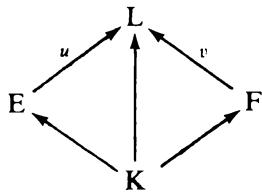
\includegraphics[keepaspectratio]{images/part001_6a404f81.jpg}}\\
FIG. 1.

In agreement with the general definitions (E, IV, p.~6) an isomorphism of a composite extension \((L, u, v)\) of E and F onto a composite extension \((L', u', v')\) of E and F is a K-isomorphism \(\varphi\) of L onto \(L'\) such that \(u' = \varphi \circ u\) and \(v' = \varphi \circ v\) .

Let \((\mathbf{L}, u, v)\) be a composite extension of \(\mathbf{E}\) and \(\mathbf{F}\) . The K-linear mapping \(w\) of \(\mathbf{E} \otimes_{\mathbf{K}} \mathbf{F}\) into \(\mathbf{L}\) which sends \(x \otimes y\) to \(u(x)v(y)\) is a K-algebra homomorphism; in this No.~we shall denote it by \(u * v\) . Its image is the subring of \(\mathbf{L}\) generated by \(u(\mathbf{E}) \cup v(\mathbf{F})\) .

PROPOSITION 4. --- Let E, F be two extensions of K.

\begin{enumerate}
\def\labelenumi{\alph{enumi})}
\item
  Let \((\mathbf{L}, u, v)\) be a composite extension of \(\mathbf{E}\) and \(\mathbf{F}\) ; then the kernel \(\mathfrak{p}\) of the homomorphism \(u * v\) of \(\mathbf{E} \otimes_{\mathbf{K}} \mathbf{F}\) into \(\mathbf{L}\) is a prime ideal.
\item
  Let \(\mathfrak{p}\) be a prime ideal of \(E \otimes_{K} F\) ; then there exists a composite extension \((L, u, v)\) of \(E\) and \(F\) such that \(\mathfrak{p}\) is the kernel of \(u * v\) , and any two such composite extensions are isomorphic.
\end{enumerate}

Assertion a) follows from the fact that the kernel of a homomorphism of a ring into a field is a prime ideal (I, p.~116-117).

Let \(\mathfrak{p}\) be a prime ideal of \(E \otimes_{K} F\) , \(A\) the quotient ring \((E \otimes_{K} F)/\mathfrak{p}\) and \(L\) the field of fractions of \(A\) . For \(x \in E\) (resp. \(y \in F\) ) we denote by \(u(x)\) (resp. \(v(y)\) ) the residue class mod \(\mathfrak{p}\) of \(x \otimes 1\) (resp. \(1 \otimes y\) ). Then \(u\) (resp. \(v\) ) is a K-homomorphism of \(E\) (resp. \(F\) ) into \(L\) and \(u(E) \cup v(F)\) generates \(A\) as a ring, hence \(L\) as a field. Therefore \((L, u, v)\) is a composite extension of \(E\) and \(F\) ; we see at once that \(u * v\) is the canonical homomorphism of \(E \otimes_{K} F\) into \(L\) , and its kernel is thus equal to \(\mathfrak{p}\) .

Let \((L', u', v')\) be a composite extension of E and F such that the kernel of \(u' * v'\) is equal to p.~Since \(u * v\) and \(u' * v'\) have the same kernel, there exists an isomorphism \(\psi\) of A onto the image A' of \(u' * v'\) , characterized by \(u' * v' = \psi \circ (u * v)\) . But A' is the subring of L' generated by \(u'(E) \cup v'(F)\) , hence \(L'\) is the field of fractions of \(A'\) . Therefore \(\psi\) extends to an homomorphism \(\varphi\) of L onto \(L'\) and it is clear that \(\varphi\) is an isomorphism of \((L, u, v)\) onto \((L', u', v')\) .

Remark. --- If p and \(p'\) are two distinct prime ideals of \(E \otimes_{K} F\) , the corresponding composite extensions of E and F (constructed by the procedure of the above proof) are not isomorphic. However, they may nevertheless be isomorphic as extensions of K (V, p.~146, Ex. 2).

COROLLARY. --- There exist composite extensions of E and F.

For since the commutative ring \(E \otimes_{K} F\) is not reduced to 0, it has prime ideals: Krull's theorem (I, p.~104) proves the existence of maximal ideals and every maximal ideal is prime.

We can make this corollary more precise as follows. Let \((\mathrm{E}, u)\) and \((\mathrm{F}, v)\) be two extensions of K; choose a maximal ideal m of the commutative ring \(E \otimes_{K} F\) and put \(L = (E \otimes_{K} F)/m\) ; then L is an extension of K. For \(x \in E\) write \(u'(x)\) for the residue class of \(x \otimes 1 \mod m\) and similarly put \(v'(y)\) for the residue class of \(1 \otimes y \mod m\) for all \(y \in F\) . We then have a commutative diagram of field homomorphisms

\pandocbounded{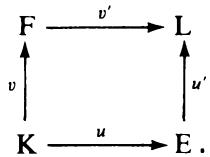
\includegraphics[keepaspectratio]{images/part001_e6455da9.jpg}}

By replacing \((L, u')\) by an isomorphic extension of E we may suppose that L contains E as subfield and that \(u'\) is the canonical injection of E in L. By changing notation we thus obtain the following scholium:

SCHOLIUM. --- Let K and E be two fields and u a homomorphism of K into E. If K' is a field containing K as subfield, there exists a field E' containing E as subfield and a homomorphism u' of K' into E' extending u.
% semantic-fragments: legacy-input-seam
\relax{}
